The Canada-France-Hawaii Telescope Lensing Survey (CFHTLenS) represented a
major step forward for the field of weak gravitational lensing, in terms of
improved accuracy in data reduction \citep{CFHTLenS-data}, the implementation
of PSF-Gaussianised matched multi-band photometry
\citep{CFHTLenS-photoz}, cross-correlation clustering analysis between
photometric redshift slices to verify tomographic redshift distributions
\citep{CFHTLenS-2pt-tomo}, accurate calibrated shape measurements
\citep{CFHTLenS-shapes} and a full suite of informative systematic tests to
select a clean data set \citep{CFHTLenS-sys}. Since the public release
of this survey in 2013, the community has continued to scrutinise and advance
our understanding of CFHTLenS by identifying a number of areas where analyses
could improve:
%
\begin{itemize}
%
 \item{\citet{2016MNRAS.463.3737C} identified significant biases in the tomographic
photometric redshift distributions using a more effective clustering analysis,
in comparison to \citet{CFHTLenS-2pt-tomo}, by incorporating newly overlapping
spectroscopic data from the Sloan Digital Sky Survey.  The conclusion of this
work was that any re-analysis of CFHTLenS should include systematic error terms
to account for bias and scatter, with a prediction that accounting for these
biases would be {\it reduce} the recovered amplitude of $\sigma_8$ by $\sim
4$\%. }
%
\item{ The CFHTLenS tomographic cosmological analysis was then revisited by
\citet{joudaki/etal:2016} in order to include a full redshift error analysis
based on the results from \citet{2016MNRAS.463.3737C}.  The impact of
correcting for these biases, including their associated errors, served to
reduce the overall constraining power of the survey and hence also the tension
between CFHTLenS and CMB constraints.}
%
 \item{\citet{2016arXiv160100115A} used the stringent COSEBI statistic
\cite{COSEBIs} to identify significant non-lensing B-mode distortions when the
CFHTLenS data was split into tomographic slices.}
%
\item{\citet{2015MNRAS.454.3500K} showed that the CFHTLenS shear calibration
corrections derived in \citet{CFHTLenS-shapes} were underestimated as a result
of an imperfect match between the galaxy populations in the data and image
simulations.}
%
\item{\citet{2016arXiv160605337F} demonstrated that the CFHTLenS data would
have been subject to a weight bias that favours galaxies that are more
intrinsically oriented with the point-spread function.  They also showed that
the impact of calibration selection biases, that were not considered in
\citet{CFHTLenS-shapes}, would have lead to the over-correction of
multiplicative shear bias in the CFHTLenS analyses, by a few percent.}
%
\item{\citet{joudaki/etal:2016} updated the CFHTLenS covariance matrices using
larger-box numerical simulations that were less subject to the lack of power on
large scales.}
\item{\cite{2012ApJ...761..152T} provided a more accurate non-linear power
spectrum correction than that used in the original CFHTLenS analyses, and the
halo model from \cite{2015MNRAS.454.1958M} allowed for simultaneous modelling
of baryonic modifications to the non-linear power spectrum.} 
%
\end{itemize}
%
All these advances in our understanding were incorporated and accounted for in
the recent KiDS cosmic shear analysis \citep{KiDS-450} which reports a $2.3
\sigma$ tension with Planck.  Efforts are now underway to fully re-analyse
CFHTLenS using the advanced KiDS analysis pipeline with revised shape
measurements and calibrations for the shear and photometric redshifts.  Until
this analysis is complete we note that these known shortcomings with the
original CFHTLenS results impact in different ways the cosmological conclusions
that one can draw from the survey.  As CFHTLenS has similar statistical power
to current weak lensing surveys, however, it nevertheless provides a very
useful testbed with which to demonstrate the impact of adopting different
approximations when constraining cosmological parameters.

\ch{New stuff here - see if you approve - edit and then de-purple it!}

\ch{In this work, we focus on the weak-lensing power spectrum projection, and
assess the impact of various approximations on cosmological constraints from
CFHTLenS. We re-analyse the 2D CFHTLenS measurement of the two-point shear correlation function $\xi_\pm(\theta)$ from \cite{CFHTLenS-2pt-notomo}, which is
given by}
\begin{equation}
\xi_\pm^{ij}(\theta) = \frac{1}{2\pi}\int_0^\infty \d\ell \,\ell \,P^{ij}_\gamma(\ell) \, J_{0,4}(\ell \theta) \, , 
\label{eqn:xiGG}
\end{equation}
\ch{where $J_{0,4} (\ell \theta)$ is the zeroth (for $\xi_+$) or fourth (for $\xi_- $) order Bessel function of the first kind and $P_\gamma(\ell)$ is the shear power spectrum at angular wave number $\ell$ which can be related to the underlying matter power spectrum through equation~\ref{eq:P_ell_limber1} when adopting a first-order extended Limber approximation, or equation~\ref{eq:P_ell_limber2} when adopting a second-order extended Limber approximation \citep[for more details see][and references therein]{miraldaescude:1991, kaiser:1992, bartelmann/schneider:2001}.  }

\ch{On a sphere, correlation functions cannot be related to the power spectrum by a Hankel transform in equation~\ref{eqn:xiGG}, as the power spectrum is not defined for non-integer $\ell$ \citep[see][for alternative spherical-sky formulae for the two-point correlation function]{2005PhRvD..72b3516C}.  As we have shown in section~\ref{sec:comp} that the spherical second-order extended Limber approximation provides a percent-level precision representation of the full spherical projection for $\ell > 3$, we do not present predictions for the two-point shear correlation function using the full spherical projection, instead choosing the spherical second-order extended Limber approximation (Ext2Sph) as our `truth' in this case.}

\ch{Figure.~\ref{fig:xi_pm_K16} presents the two-point correlation functions $\xi_+$ (left) and $\xi_-$ (right) using the different cases for the shear power spectrum listed in Table~\ref{tab:cases}. The adopted CFHTLenS redshift distribution and fiducial cosmological model are the same as in Figure.~\ref{fig:Cl_cases}.   }


\begin{figure}

  \begin{center}
    \resizebox{1.0\hsize}{!}{
      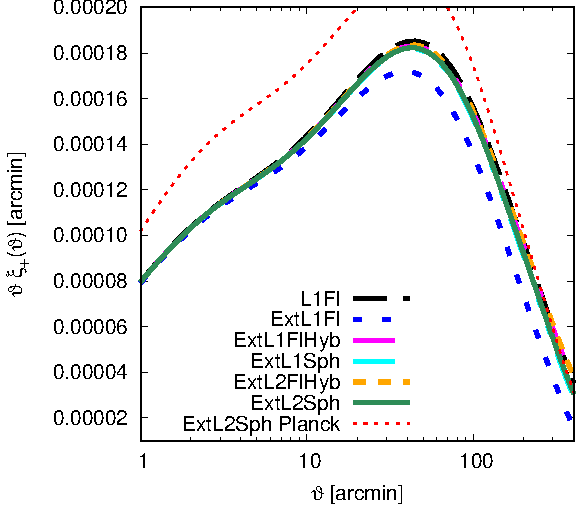
\includegraphics{figures/xi_p_comp}
      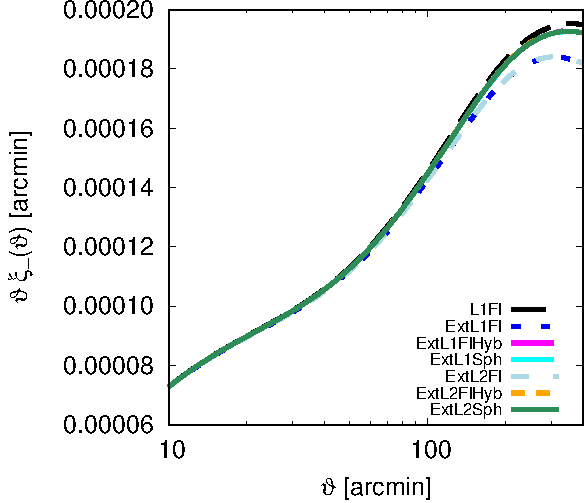
\includegraphics{figures/xi_m_comp}
    }

    \resizebox{1.0\hsize}{!}{
      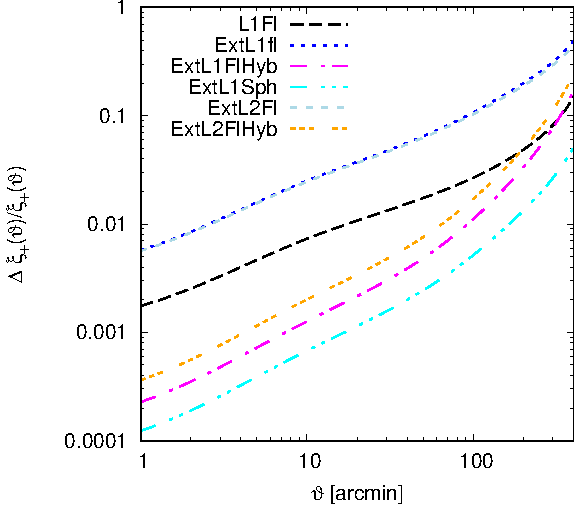
\includegraphics{figures/xi_p_delta}
      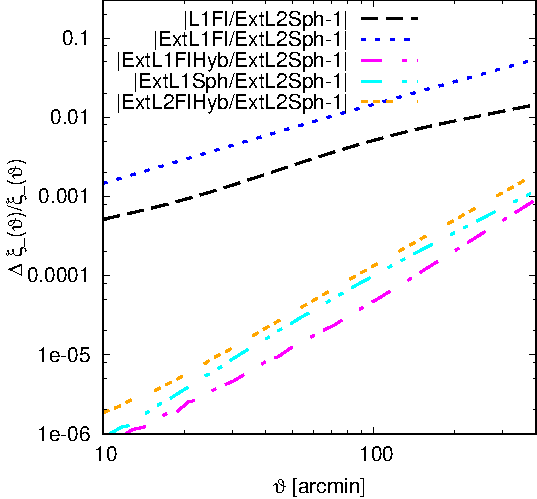
\includegraphics{figures/xi_m_delta}
    }
  \end{center}

  \caption{Shear correlation functions $\xi_+$ (\emph{left}) and $\xi_-$ (\emph{right}).
    The lower panels shows the relative differences to the case Ext2Sph,  see Table \ref{tab:cases} for the different
    approximations and their symbols.
    \mk{Probably remove ExtL1Fl, ExtL2Fl, we already showed for $P_\kappa$ that they are worse than standard
    Limber.}
    \ch{ExtL2Fl isn't in the table - so yes agreed to remove that from both plots}
    \ch{I'd keep the ExtL1Fl, just incase someone is daft enough to do that approximation one day.}
    %\cite{CFHTLenS-2pt-notomo}; the theoretical predictions correspond to the best-fit parameters with
    %$\Omega_{\rm m} = 0.279$ and $\sigma_8 = 0.79$, except the red dashed curve with adapts a Planck-best fit
    %normalisation $\sigma_8 = 0.83$.
  }

  \label{fig:xi_pm_K16}

\end{figure}


For consistency, we adopt the same priors and non-linear power spectrum corrections\footnote{As
an example of more significant effects that need to be accounted for, when using the
revised non-linear power spectrum of \cite{2012ApJ...761..152T} in place of
\cite{2003MNRAS.341.1311S}, there is a decrease of $0.6 \sigma$ with $\sigma_8
(\Omega_{\rm m}/0.27)^{0.6} =0.768^{+0.029}_{-0.031}$.} from
\cite{2003MNRAS.341.1311S} as the original \cite{CFHTLenS-2pt-notomo} analysis.
For a first-order standard Limber flat-sky approximation (L1Fl) we find
$\sigma_8 (\Omega_{\rm m}/0.27)^{0.6} =0.787^{+0.031}_{-0.033}$. For a
second-order extended Limber flat-sky approximation we find $\sigma_8
(\Omega_{\rm m}/0.27)^{0.6} =X^{+X}_{-X}$, a negligible change of
$X\sigma$. 

Table \ref{tab:CFHTLenS_Sigma8} lists the mean and 68\% credible interval for
$\sigma_8 (\Omega_{\rm m}/0.3)^{0.6}$ for the various approximations to the
lensing power spectrum projections listed in Table~\ref{tab:cases}

\renewcommand{\baselinestretch}{1.5}
\begin{table}

  \label{tab:CFHTLenS_Sigma8}

  \caption{Mean and 68\% credible interval for 
  $\sigma_8 (\Omega_{\rm m}/0.3)^{0.6}$ for various approximations to the lensing
  power spectrum projections.}

  \begin{tabular}{lcc} \hline
  ID         & $\sigma_8 (\Omega_{\rm m}/0.27)^{0.6}$ & $\sigma_8 (\Omega_{\rm m}/0.3)^{0.6}$\\ \hline
  L1Fl       & $0.787^{+0.031}_{-0.033}$ & $0.739^{+0.029}_{-0.031}$ \\
  ExtL1FlHyb & $0.788^{+0.031}_{-0.033}$ & $0.740^{+0.029}_{-0.031}$ \\
  ExtL2Sph   & $0.789^{+0.031}_{-0.032}$ & $0.740^{+0.029}_{-0.030}$ \\ \hline
  \end{tabular}

\end{table}
\renewcommand{\baselinestretch}{1}


